\documentclass[12pt]{article}
\usepackage[letterpaper, margin=1in]{geometry}
% \usepackage[dvipsnames]{xcolor}
% \usepackage{xcolor}
\usepackage{graphicx}
\usepackage{subcaption}
\graphicspath{{./figures/}}
\usepackage{hyperref}
\hypersetup{
    colorlinks=true,   
    urlcolor=blue,
}
\usepackage{parskip}
\usepackage{amsmath}
\usepackage{titlesec}
% \usepackage{listings}
\usepackage[numbered, framed]{matlab-prettifier}

% \definecolor{backgroundColour}{rgb}{0.95,0.95,0.92}
% \lstset{
%     % frame=single,
%     captionpos=b,   % sets the caption-position to bottom
%     breaklines=true,
%     numbers=left,
%     % numbersep=5pt,
%     numberstyle=\tiny\color{gray},
%     tabsize=2,
%     basicstyle=\ttfamily\scriptsize,
%     showspaces=false,
%     showstringspaces=false,
%     backgroundcolor=\color{backgroundColour},
%     keywordstyle=\color{Magenta},
%     identifierstyle=\color{MidnightBlue},
%     commentstyle=\color{Green},
%     stringstyle=\color{Maroon}}


\titleformat*{\section}{\large\bfseries}
%\allowdisplaybreaks

% remove vertical spacing above top figure
\makeatletter
\setlength{\@fptop}{0pt}
\makeatother
%

\renewcommand{\thesubsection}{\thesection.\alph{subsection}}

\title{COMPENG 3SK3 Project 1 Report}
\author{
    Raeed Hassan \\
    hassam41 \\
}

\begin{document}

\maketitle
\clearpage

\section{Pseudo Code}
\begin{lstlisting}[style=Matlab-editor]
% initialize singles

% divide series into 4 parts for each parallel processor

% evaluate each part using a parallel processor
p1 = increment N, divide 1/N and alternate between addition and subtraction to sum
p2 = increment N, divide 1/N and alternate between addition and subtraction to sum 
p3 = increment N, divide 1/N and alternate between addition and subtraction to sum 
p4 = increment N, divide 1/N and alternate between addition and subtraction to sum 

% sum all parts for final result
sum = p1_sum + p2_sum + p3_sum + p4_sum
\end{lstlisting}
\section{Simulation}
The simulation implementation is slightly different as it puts each operation on a parallel processor instead of splitting up terms equally to do on each processor. The method described in the pseudo code is preferred as the parallel processors will not be dependent on each other (essentially becoming serial), but this simulation is easier to understand.

\lstinputlisting[style=Matlab-editor, firstline=3, lastline=32]{../project1.m}
\section{Design Decision}
The pseudo code design splits groups of terms and executes these terms on serially on parallel processors. This allows each processor to function independently from each other. The simulation instead puts each individual operation onto a parallel processor and performs operations for any term N on all parallel processors. This was done to make coding the problem simpler, as performance was not a concern for such a simple program.
\section{Questions}

% Can you achieve, in the IEEE 32-bit floating number system, any high precision you desire by summing up the first N terms of the series and by running the summation program for a sufficiently large N? Explain your answer.
\subsection[q4a]{High Precision}
It is not possible to achieve any high precision you desire by summing up the first N terms of the series as the IEEE 32-bit floating number system inherently has precision limitations. The sum of the series, which would also be represented in the IEEE 32-bit floating number system, would inherit the same precision limitations of the system and would have an upper-bound limit on its precision.

% With respect to the IEEE 32-bit floating number system, what is the minimum N value such that 1/N becomes too small to be representable? What is the minimum N value such that 1/(N-1)-1/N becomes too small to be representable?  What is the minimum N value such that 1/N is smaller than machine precision?  What is the minimum N value such that 1/(N-1)-1/N is smaller than machine precision.
\subsection[q4b]{Minimum N}
The minimum N value such that 1/N becomes too small to be representable is N = $2^{128}$. 

The minimum N value such that 1/(N-1)-1/N becomes too small to be representable is N $= 2^{24}+4$. 

The minimum N value such that 1/N is smaller than machine precision is N = $2^{23}+1$.

The minimum N value such that 1/(N-1)-1/N is smaller than machine precision is 2898.



% For your algorithm to sum the first N terms of the alternating harmonic series, plot the curve of numerical error against N. Explain the behavior of the error curve. To compute the numerical error, the reference (ground truth) is the Matlab double precision value ln2 = Matlab function log(2) = 0.693147180559945....
\subsection[q4c]{Numerical Error Against N}
The numerical error against N is plotted in Figure~\ref*{fig:q4c}. The error curve plots the numerical error against N from N = 1 to N = $2^{10}$. We can observe the error curve decreases as the value of N increases. This means the value of the sum of the alternating harmonic series gets closer to $\ln 2$ as the number of terms in the series increases.
\begin{figure}[htp]
\centering
\caption{Numerical Error against N}\label{fig:q4c}
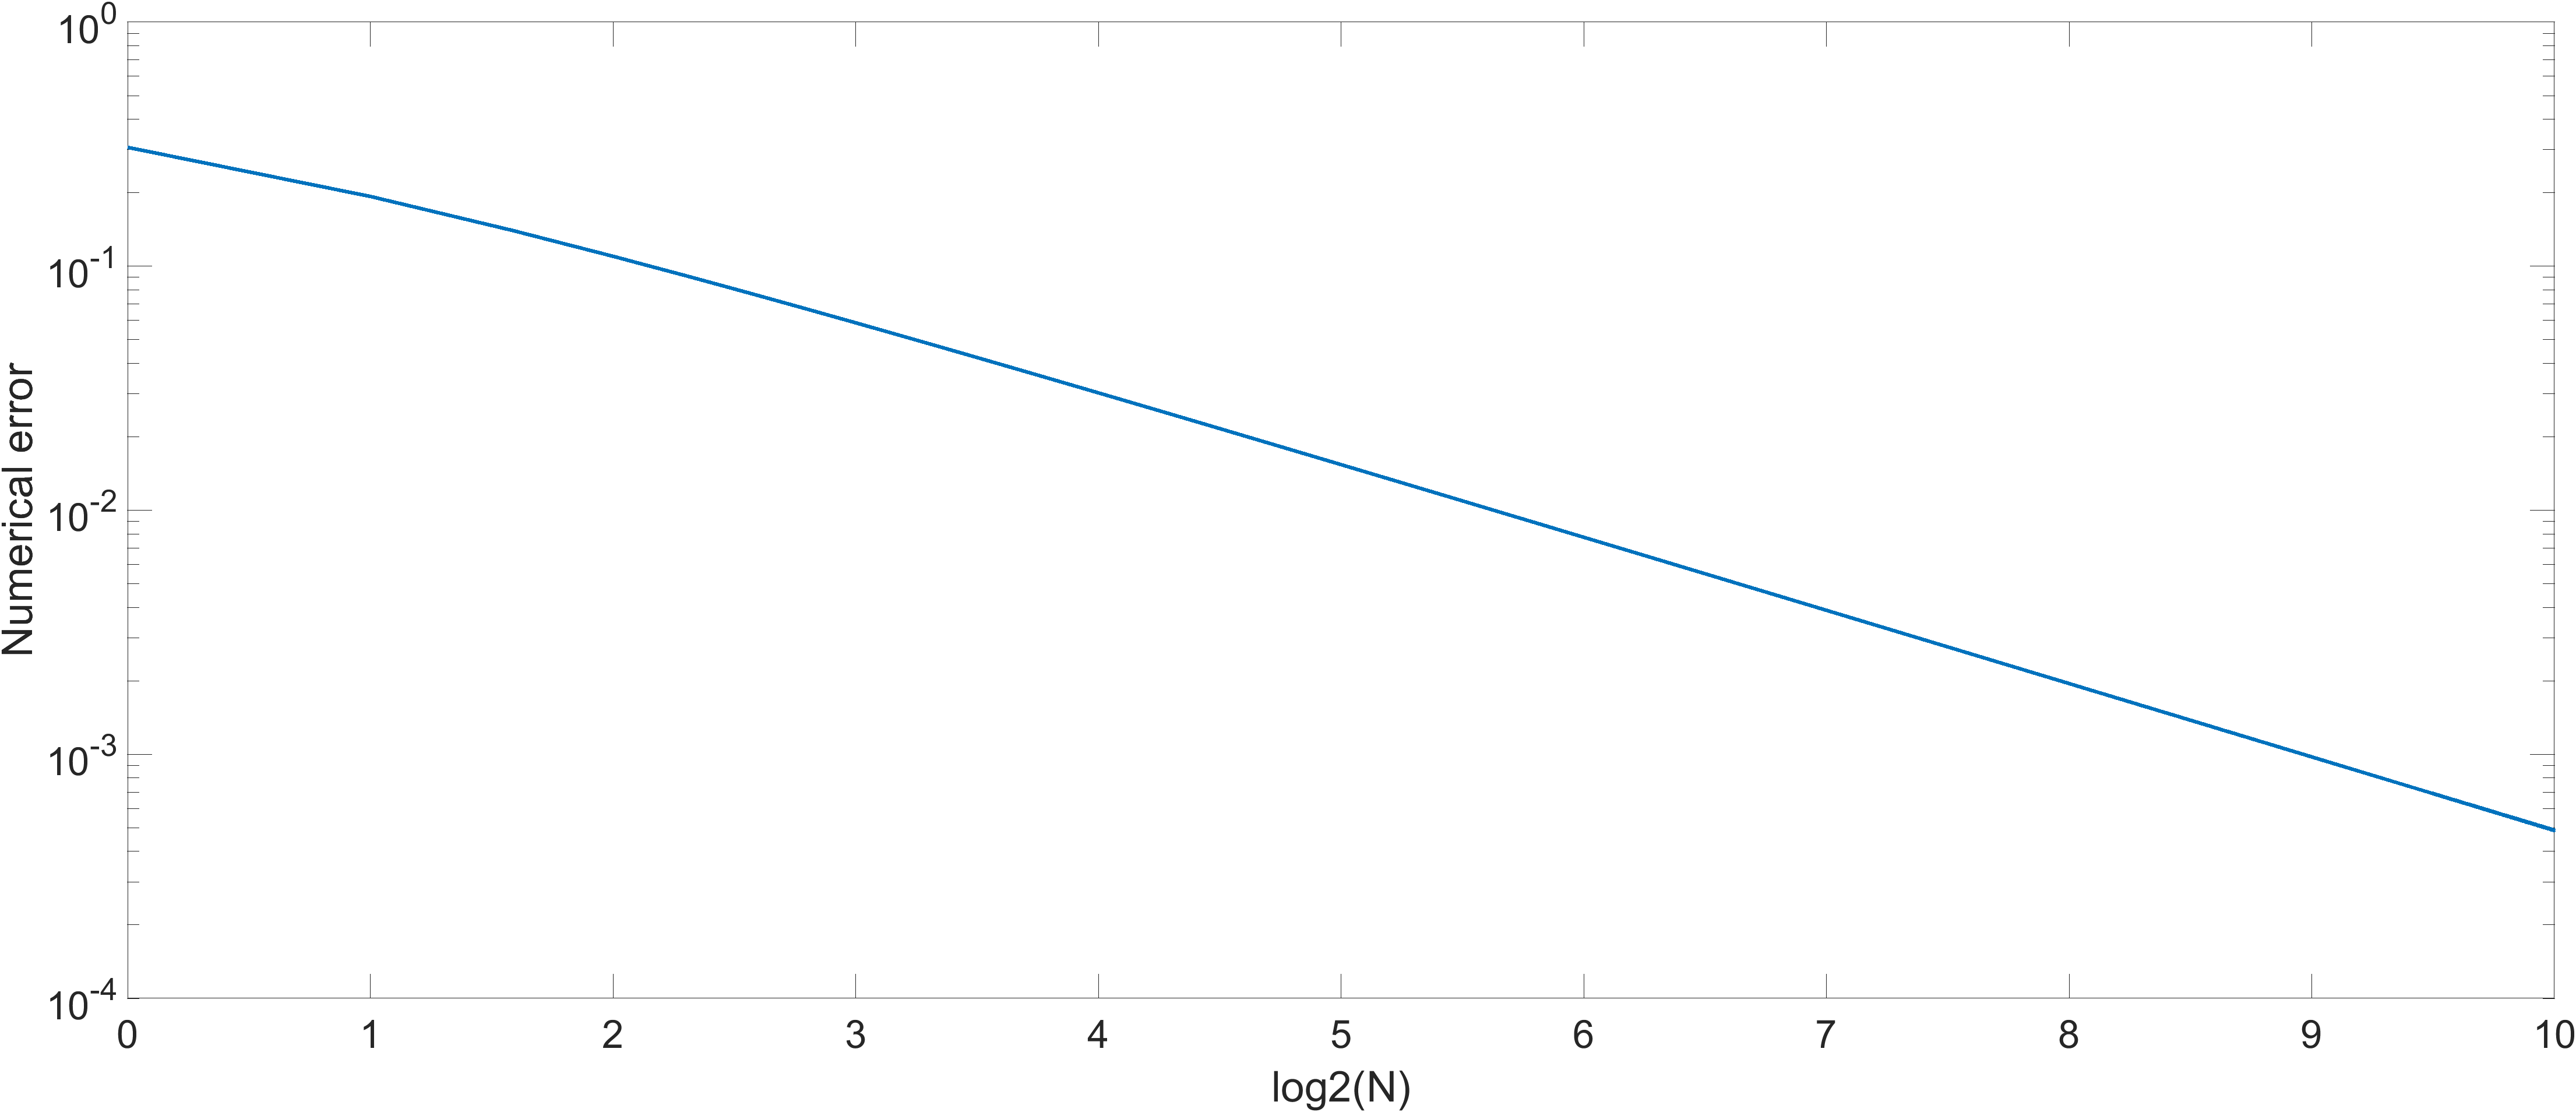
\includegraphics[width=\textwidth]{q4c.png}
\end{figure}

% Does your algorithm achieve the highest possible precision? If not, suggest a possible way to improve the precision.
\subsection[q4d]{Highest Possible Precision}
This algorithm does not achieve the highest possible precision. For example, precision is lost during the accumulation process as the result after each summation is truncated. The algorithm could be improved by implementing a method to reduce numerical error by using the Kahan summation algorithm, also called compensated summation.

This method works by keeping maintaining a separate variable which accumulates the error of the summation to compensate the sum at the end.
\end{document}